
\chapter{On the relationship between Arctic winter precipitation and minimum sea ice extent}
\label{chap:winter_prec}

This chapter is to be submitted to \textit{Geophysical Research Letters} as

\hangbibentry{Hamman_2016f}

\section*{Abstract}

Over the past three decades, the Arctic has experienced large declines in summer sea ice cover, permafrost extent and spring snow cover, as well as increases in winter precipitation.
This study explores the relationship between declining Arctic sea ice extent and early winter precipitation across the high-latitude Arctic land masses.
The first part of this paper presents the observed relationship between sea ice extent and winter precipitation.
Using satellite estimates of sea ice extent and precipitation data based on a combination of in-situ observations and global reanalyses, we show that early winter precipitation is negatively correlated with summer sea ice extent and that this relationship is strongest before the year 2000.
After 2000, around the time sea ice extent minima began to decline most rapidly, the relationship between sea ice extent and early winter precipitation degenerates.
This indicates that other processes are driving changes in sea ice extent and winter precipitation.
We hypothesize that the observed correlations between sea ice extent and high winter precipitation are related to anomalous patterns in ocean evaporation and sea ice extent in the fall.
To better understand the physical mechanisms driving the observed changes in the Arctic climate system and the sensitivity of the Arctic climate system to declining sea ice, we have used the fully-coupled Regional Arctic System Model (RASM) to simulate three distinct sea ice climates.
The first climate represents normal sea ice extent, while the second and third represent reduced summer sea ice extent.
The second part of this paper analyzes these three RASM simulations, in conjunction with our observation-based analysis, to understand the relationship between poleward moisture transport, sea ice extent, evaporation from the Arctic Ocean, and precipitation.
We will present the RASM-simulated Arctic water budget and demonstrate the role of sea ice extent in driving winter precipitation anomalies.
Finally, we use the Self-Organizing Map (SOM) machine learning technique to identify characteristic patterns of ocean evaporation, sea ice extent, and polar cap convergence that contribute to anomalies in early winter precipitation.

\section{Introduction}
\label{sec:intro_ch5}

In the past three decades, the Arctic region has experienced unprecedented changes in key cryospheric processes.
Rapid declines in sea ice cover have been accompanied by reductions in permafrost extent and spring snow cover, as well as increases in winter precipitation and winter snow accumulations \citep{Kohler_2006,Callaghan_2011,Bulygina_2009}.
These combined changes have had a marked impact on the regional and global climate systems.
Driving much of these changes has been a regional warming trend that is nearly twice as large as the global mean \citep{Serreze_2006c,Screen_2010}.
This disparity in temperature increases is often referred to as Arctic Amplification and is largely explained by the ice-albedo feedback \citep{Curry_1995}.
While this is likely the primary mechanism that leads to rapid warming in the Arctic, other, secondary feedback processes are also at play.
One such feedback process relates the state and fluxes of the Arctic Ocean (sea surface temperatures or SSTs, sea ice cover, evaporation) to precipitation over land, which modulates winter snow cover and permafrost health.

Observational evidence of an amplified hydrologic cycle \citep{Stocker_2005} has been found in the form of increasing precipitation \citep{Rawlins_2006}, runoff \citep{Peterson_2002}, and winter snow accumulations \citep{Kohler_2006,Bulygina_2009}.
While global average precipitation is expected to increase following a response to warming via the Clausius-Clapeyron relationship \citep[e.g. ][]{Held_2006,Stephens_2008,Byrne_2015}, precipitation increases in the Arctic are expected to exceed the global average \citep{Stocker_2005}.
Analysis of the collection Earth system models (ESMs) in the Coupled Model Intercomparison Project Phase 5 \citep[CMIP5; ][]{Taylor_2012} by \citet{Bintanja_2014} indicates that annual precipitation changes in the Arctic may exceed 50\%, with the largest relative increases in the winter over the Arctic Ocean when precipitation has typically been low.
\citet{Bintanja_2014} also identify that most of these changes are due to precipitation sourced from enhanced local evaporation related to retreating sea ice.
This somewhat contradicts previous work that suggested increased poleward moisture transport as the main driver of Arctic precipitation increases.
Combined with the large intermodel spread of precipitation changes in their study, this contradiction brings into question the sensitivity of the response of Arctic precipitation to reduced sea ice in modern ESMs.
ESMs, along with statistical models, tend to poorly represent the observed decline in summer sea ice extent.
This is evidenced by the intermodel spread among the 39 ESMs analyzed by \citet{Bintanja_2014}.
In their study, changes in sea ice extent between the beginning and end of the twenty-first century ranged between 31-66\%, while changes in precipitation varied by a factor of three to four.

Conceptually, a warmer Arctic Ocean with less sea ice will lead to increased surface evaporation and may lead to enhanced divergence of moisture onto land in the form of precipitation.
Because high-latitude land areas are predominantly below freezing in the fall, increases in precipitation during this season are expected to produce deeper snow packs.
This process would then act to insulate the underlying ground during winter and suppress cold season cooling of high-latitude permafrost \citep{Osterkamp_1999,Zhang_2005,Lawrence_2010}.
Further permafrost degradation may be attributed to earlier spring snow melt driven by regional warming and possibly by increased surface infiltration of warm meltwater \citep{Lawrence_2010}.

How the Arctic climate will respond to such large temperature and sea ice changes has been at the forefront of recent studies \citep[e.g. ][]{Kazutoshi_2014,Simmonds_2014,Wegmann_2015,Vihma_2014}.
Here, we investigate the relationship between Arctic winter precipitation, ocean evaporation, and sea ice extent to better understand the terrestrial precipitation response to the ongoing sea ice decline.
Our a priori hypothesis is that the reductions in sea ice extent would lead to increases in evaporation from the central portions of the Arctic Ocean and precipitation over land during the fall and early winter months.
We explore this hypothesis using three simulations spanning a range of sea ice climates from a fully-coupled regional ESM described in Section \ref{sec:data_models_ch5}.
In Section \ref{sec:results_ch5} we present our analysis of these simulations, first computing the regional freshwater budget following \citet{Serreze_2006a}, then using the Self-Organizing Map (SOM) machine learning technique for dimension reduction and pattern evaluation \citep{Kohonen_1998,Hewitson_2002}.

\section{Data and Methods}
\label{sec:data_models_ch5}

\subsection{Models}
\label{sec:models}
We use three simulations from the Regional Arctic System Model \citep[RASM; ][]{Hamman_2016a,Roberts_2015a}.
RASM is a high-resolution, fully-coupled regional ESM that has been recently developed to improve the representation of coupled Arctic processes.
RASM is comprised of individual land \citep[see ][]{Hamman_2016a}, atmosphere \citep[see ][]{Cassano_2016}, ocean \citep[see ][]{Roberts_2015a}, sea ice \citep[see ][]{Roberts_2015a}, and runoff \citep[see ][]{Hamman_2016b} components, coupled via the CESM flux coupler \citet{Craig_2011}.
In RASM, the atmosphere is forced at its lateral boundaries with the ERA-Interim Reanalysis \citep{Dee_2011} and the ocean's closed boundaries are relaxed to the climatology from \citet{Steele_2001}.
It is important to note that spectral nudging is applied to temperature and winds in RASM above 500 hPa.
From a practical perspective, this nudging means that the synoptic scale circulation patterns in all three RASM simulations closely match those of ERA-Interim \citep{Glisan_2013}.
The land, atmosphere, and runoff components in RASM are applied on a 50 km near equal area polar stereographic grid while the ocean and sea ice are applied on a 1/12$^{\circ}$ rotated pole mesh.

Each of the three RASM simulations used here were run from September 1, 1979 through December 31, 2014, although our analysis begins after a 10-year spinnup to allow for the stabilization of the ocean and sea ice components under coupled forcings.
\citet{Hamman_2016b} provide a complete description of the configuration of RASM for the baseline $RASM_{CONTROL}$ simulation.
Two sensitivity simulations, $RASM_{RSI}$ and $RASM_{RSH}$, representing intermediate and high reductions in sea ice extent are also analyzed.
The configuration of these simulations is identical to $RASM_{CONTROL}$ except in the parameterization of sea ice albedos, which is summarized in Table \ref{table:sims}.
Sea ice albedo is reduced in both simulations to promote accelerated spring sea ice melt and reduced sea ice extent in the summer and fall.
This method of altering the radiative properties of sea ice allows for fully-coupled, self-consistent simulations in RASM and avoids issues with prescribing unphysical surface conditions.

\begin{table}[]
    \centering
    \caption{Summary of RASM simulations used in this chapter.}
    \label{table:sims}
    \begin{tabular}{|l|p{4in}|}
    \hline
    \textbf{Dataset} & \textbf{Sea Ice / Ocean Configuration}                                                                                                         \\ \hline
    $RASM_{CONTROL}$    & Default RASM (see \citet{Hamman_2016b})                                                                                                          \\ \hline
    $RASM_{RSI}$         & \begin{tabular}[c]{@{}l@{}}Ocean: No changes\\ Sea Ice: Snow albedo -0.5 std. dev. of observed.\end{tabular}                                   \\ \hline
    $RASM_{RSH}$         & \begin{tabular}[c]{@{}p{3.5in}}Ocean: No changes\\ Sea Ice: No sea ice initial condition, reduced snow/ice/pond albedo -2.0 std. dev.
    \end{tabular} \\ \hline
    \end{tabular}
\end{table}

\subsection{Datasets}
\label{sec:data}
Observations of sea ice extent are taken from the National Snow and Ice Data Center (NSIDC) Weekly Sea Ice Extent product \citep{Brodzik_2013}.
Gridded precipitations observations between 1979 and 2014 are taken from CRU TS v.3.23 \citep{Harris_2014}.
We also used monthly mean precipitation data ERA-Interim \citep[referred to hereafter as ERA; ][]{Dee_2011} and NASA’s Modern-Era Retrospective Analysis for Research and Applications \citep[MERRA; ][]{Rienecker_2011}.
These two datasets, originally provided at their respective native resolution of 0.75$^{\circ}$x0.75$^{\circ}$ and 0.5$^{\circ}$ x 0.667$^{\circ}$ spatial resolutions, were resampled to RASM's land/atmosphere grid for use in this study.

\subsection{Self-Organizing Maps}
In Section \ref{sec:rasm_results}, we present results using the Self-Organizing Map \citep{Kohonen_1998,Hewitson_2002} technique.
SOMs are a useful technique for dimension reduction, allowing for the identification of unique climatological patterns.
They are are a type of unsupervised machine learning, utilizing artificial neural networks to create a lower-dimensional representation of high-dimensional datasets.
SOMs have been previously applied in studies of polar climatology to study synoptic scale atmospheric circulation \citep[e.g. ][]{Cassano_2007}, extreme weather events \citep[e.g. ][]{Cassano_2015,Glisan_2016}, and coupled ocean-atmosphere processes \citep[e.g. ][]{DuVivier_2016}.

In our analysis, we trained a 2x4 SOM, using standardized ocean evaporation anomalies north of 55$^{\circ}$ N from each of the three RASM simulations described in Section \ref{sec:models} for individual fall months (October - December) between 1985 and 2014.
In total, the training dataset was comprised of 270 months of evaporation anomalies.
Standardized anomalies were calculated using the climatology calculated from the entire analysis period.
We used a evaluation metric of Euclidean distance, a learning rate of 0.001, and a maximum number of iterations of 2000.
The shape of the 2x4 SOM was chosen to provide a sufficient number of unique patterns while maximizing the average number of samples in each pattern.
% BN: Should the training domain be limited to that of Figure 4?  % JH: I have tried that and we can go over those results. I remember them not being particularly easy to understand.
The SOM was initialized with random fields from a standard normal distribution. % BN: This doesn't mean much to people who have not used SOMs. What is the implication of this choice for initialization?
% JH: True, but since there are other ways to initialize a som, I think it is important that we state our methodology.
% BN: Are all cells independent?
% JH: No. The each month is put into an individual node.
Further details on the SOM algorithm can be found in \citet{Reusch_2005} or \citet{Cassano_2015}.

\section{Results and Discussion}
\label{sec:results_ch5}
\subsection{Observational evidence}
% Motivation and establishing a connection between sea ice extent and precipitation
Our hypothesized relationship between precipitation and sea ice extent builds on the observed interannual covariation of precipitation and sea ice extent across the central Arctic drainage basin.
Here we define the central Arctic drainage basin as the land areas draining to the core sea ice regions of the Arctic ocean, including the Siberian Shelf (mainly the Kolyma and Lena Rivers) and Canadian coast (mainly the Mackenzie River).
% BN: A figure would help in describing the central arctic. You can probably overlay this on Figure 2 or just refer to Figure 4.
Figure \ref{fig:prec_ice_ts} presents the timeseries of observed annual minimum sea ice extent and October-December precipitation in the central Arctic drainage basin from the MERRA and ERA reanalysis and CRU datasets.
Using the Spearman rank-order correlation measure \citep{Spearman_1904}, the MERRA, ERA, and CRU datasets exhibit correlations of -0.38, -0.40, and -0.52 respectively.
The observed relationship (i.e., negative correlations) is most prominent prior to 2000.
This raises the question whether the two processes are related through a physical coupling that is limited by a threshold mechanism or whether they are perhaps driven by a common forcing.

\begin{figure}
  \centering
  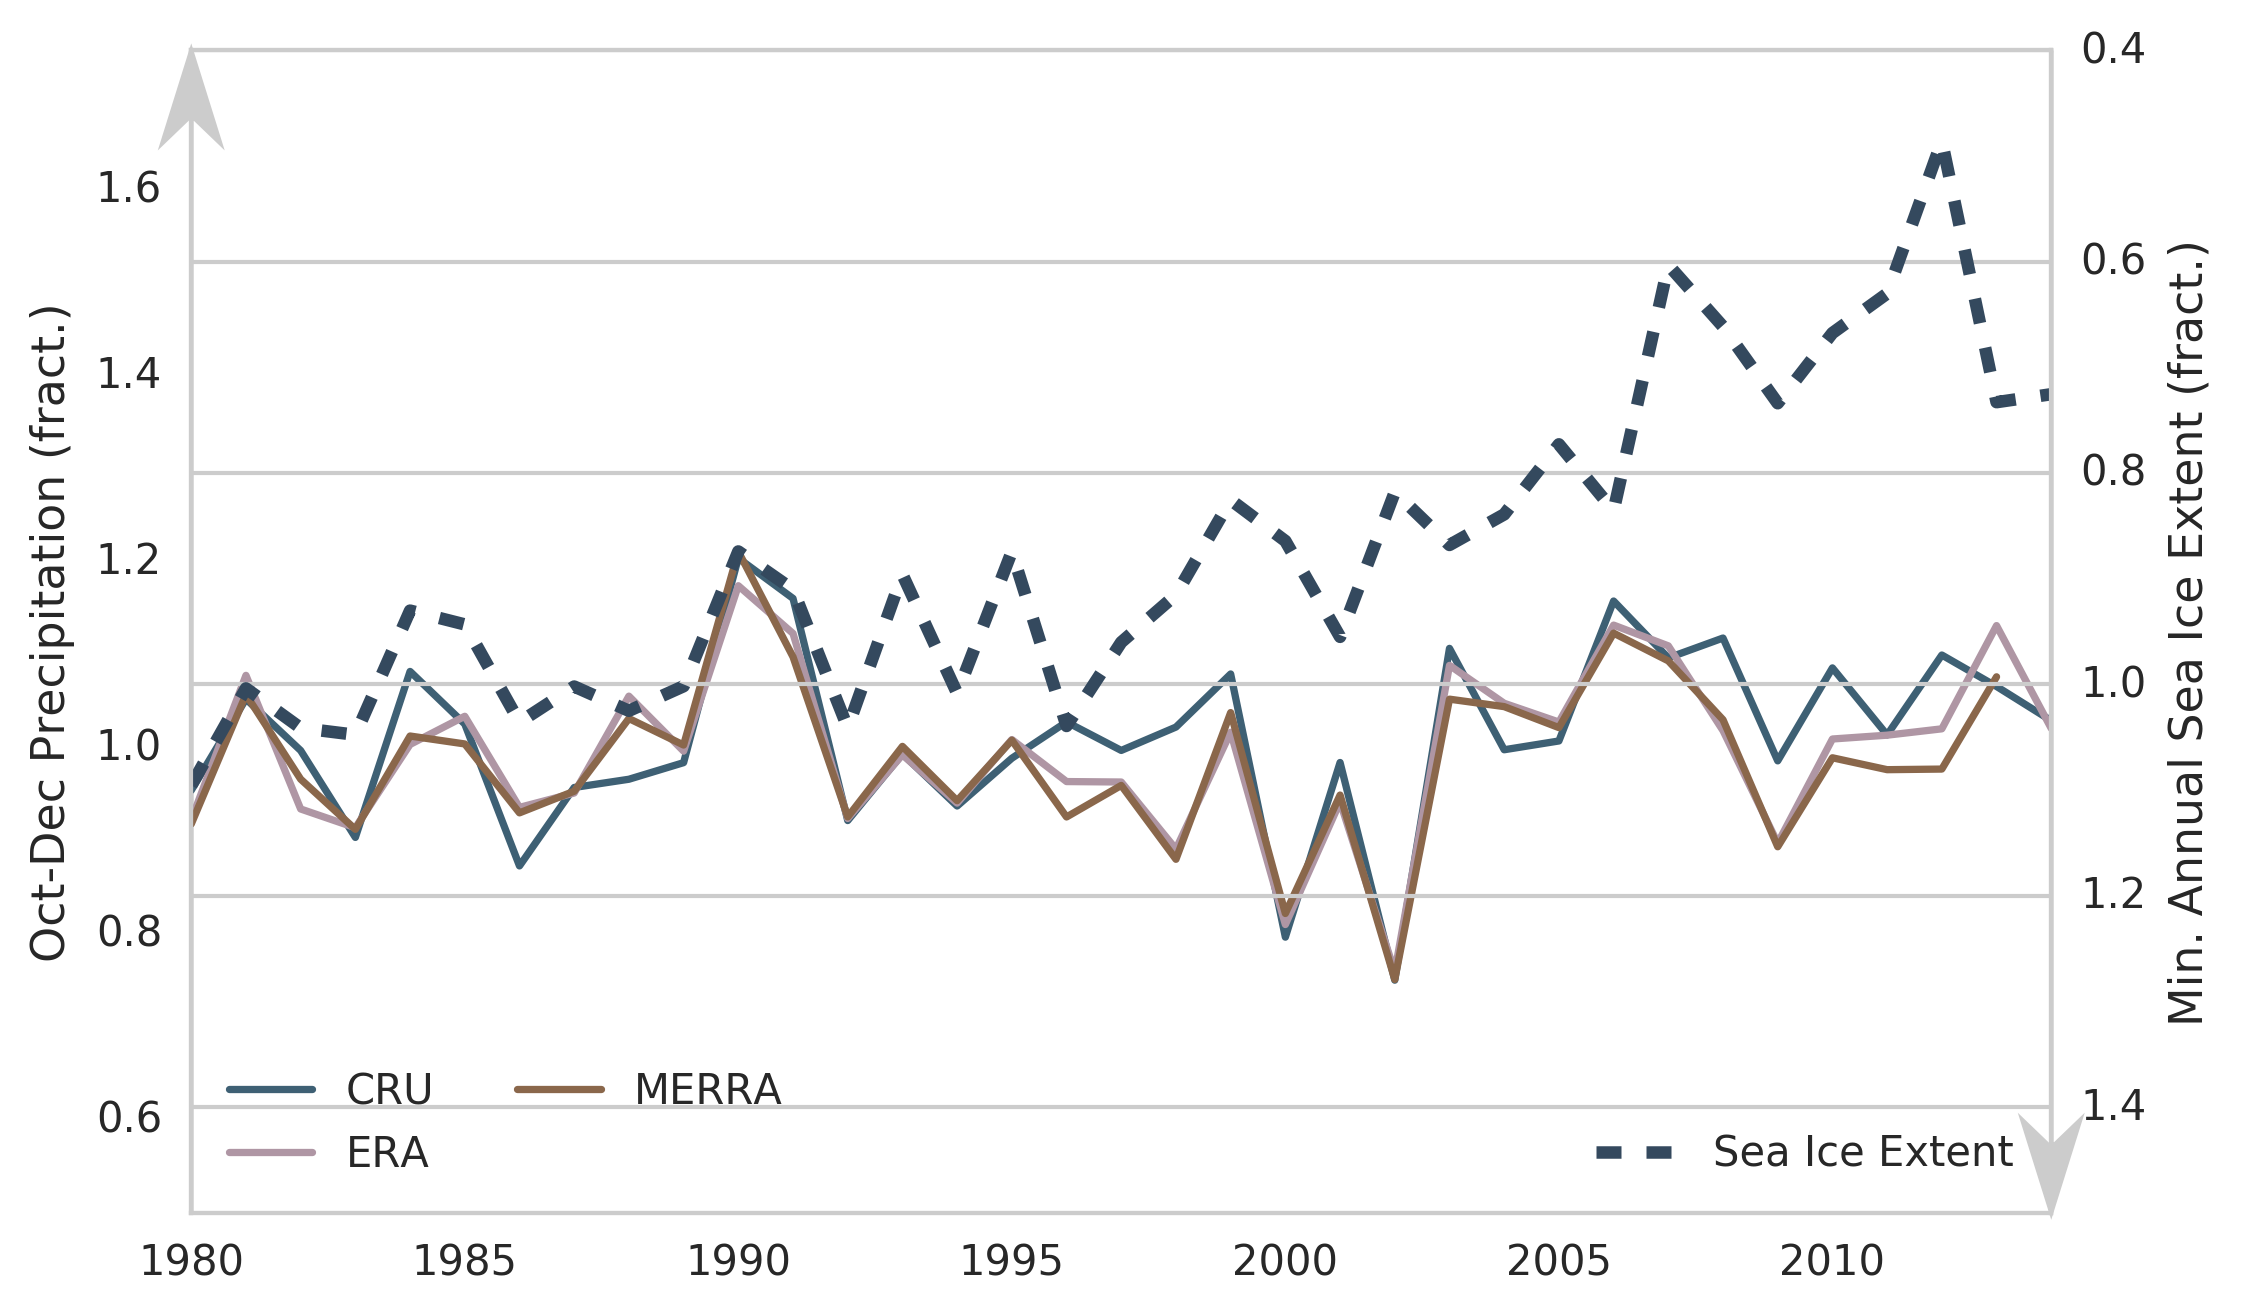
\includegraphics[width=12cm,keepaspectratio]{prec_seaice_ts}
  \caption{Timeseries (1980-2015) of fall precipitation (Oct - Dec) over the central Arctic drainage basin, (left axis) compared to minimum annual sea ice extent (right axis). Note that the right axis is inverted. Units for both axes are fraction of the 1980-1990 mean.}
  \label{fig:prec_ice_ts}
\end{figure}

Figure \ref{fig:prec_spatial_corr} shows the Spearman rank-order correlation coefficients between minimum annual sea ice extent and October-December precipitation from the CRU dataset at each grid cell within the RASM domain.
Across most of the domain, the correlations are found to be below zero, with the most negative correlations occurring across Siberia and North America.
Correlations across northern Europe are predominantly near zero or positive. % BN: But is Europe part of the central Arctic drainage as you describe it earlier? I think you need to mask these figures to ONLY show the part that is actually used in analysis (the lines in Figure 1).
% JH: I've masked the spatial figure for the RVIC drainage and just called out the northern Europe piece.
Generally, a moderately consistent relationship exists between sea ice extent and precipitation, especially in the high-latitude regions of the study domain.
In the following sections, we will investigate possible mechanisms for this relationship.

\begin{figure}
  \centering
  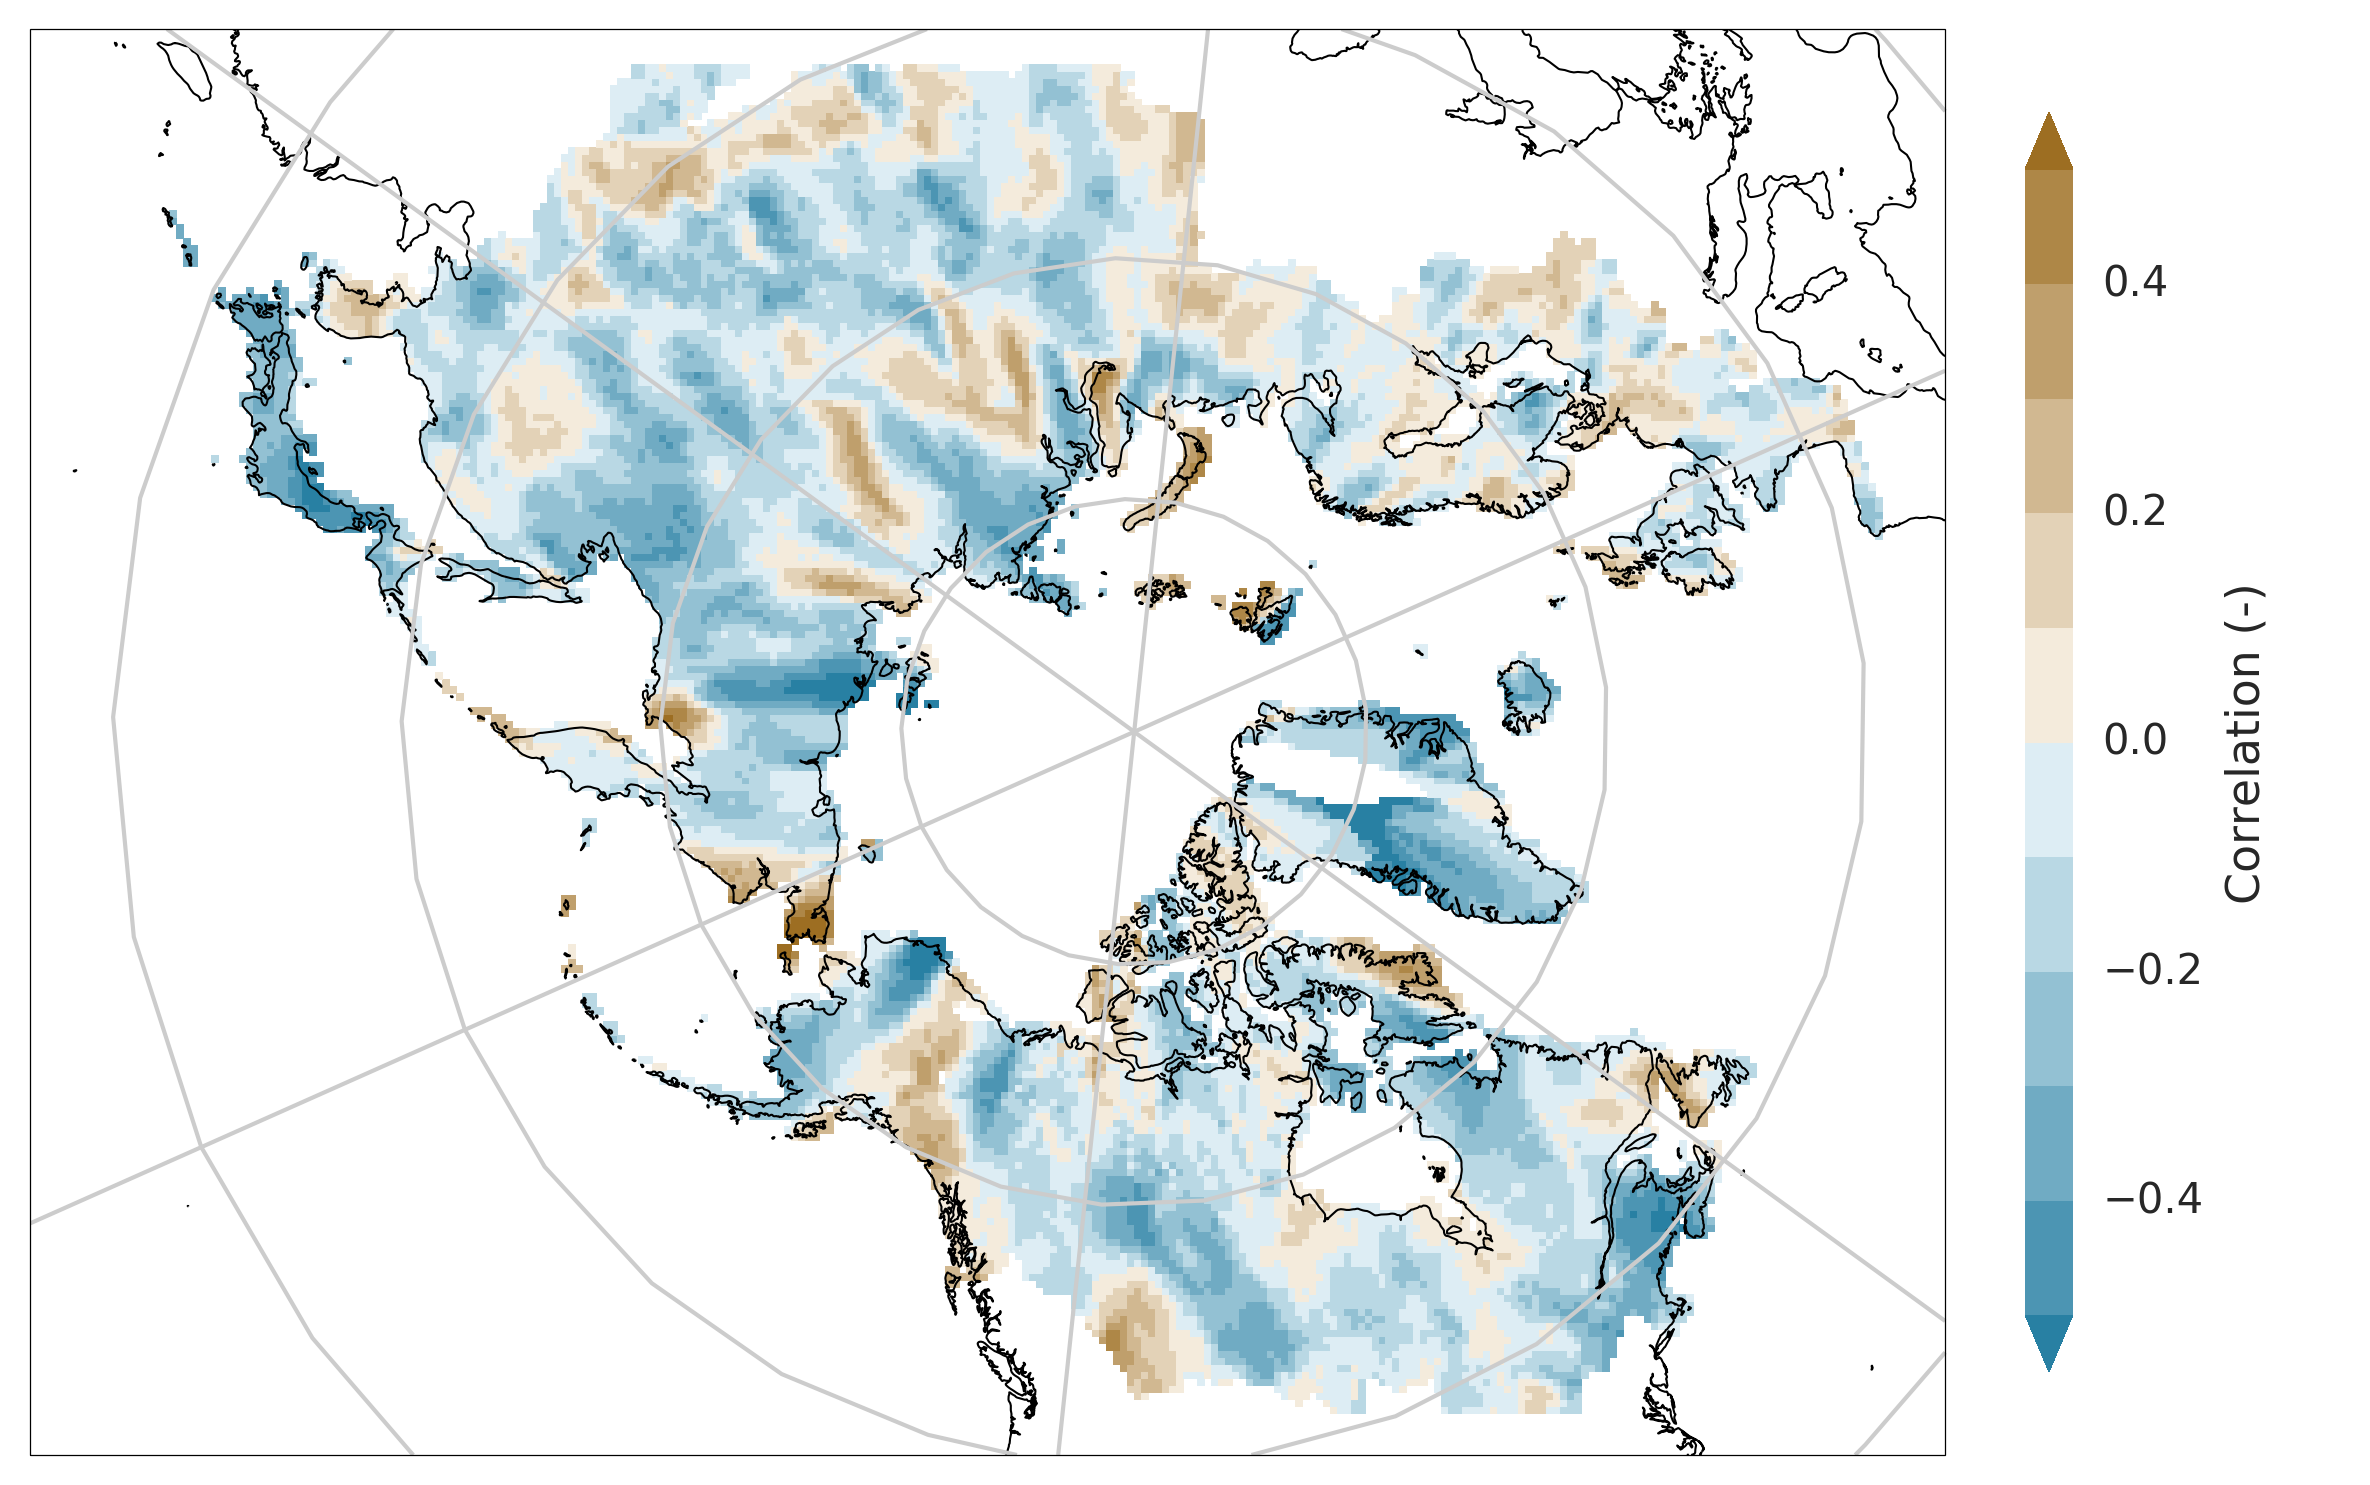
\includegraphics[width=12cm,keepaspectratio]{cru_correlation}
  \caption{Spearman rank-order correlation coefficients between observed minimum annual sea ice extent and gridded Oct-Dec precipitation from CRU. Time period 1980-2015.}
  \label{fig:prec_spatial_corr}
\end{figure}

\subsection{RASM simulations}
\label{sec:rasm_results}

% RASM sea ice sensitivity

% BN: This section needs to be beefed up.

% BN: Include some spatial maps of sea ice extents and delve a bit deeper into the results. Do we have minimum sea ice extents at the right time and in the right years (since we are using reanalysis to drive the simulation I assume so.)
% JH: This will have to be done after we submit the dissertation.
Figure \ref{fig:sea_ice_box} shows box-and-whisker plots of sea ice extent from the three RASM simulations described in Section \ref{sec:data_models_ch5} compared to the NSIDC observation-based estimates.
Compared to $RASM_{CONTROL}$, $RASM_{RSI}$ and $RASM_{RSH}$ have reductions in minimum annual sea ice extents of 16\% and 49\% respectively.
In the fall, these simulations include smaller reductions in mean sea ice cover of 3\% and 11\% respectively.
However, compared to the RASM simulations, the observations of sea ice extent demonstrate significantly more interannual variability.
Individual months can be clearly seen in \ref{fig:sea_ice_box} with the lowest values in each simulation corresponding to Octobers, the middle values corresponding to Novembers, and the highest values corresponding to Decembers.
The RASM simulations have interannual standard deviations for each of these months that are 1.6 to 3.5 times smaller than the observations.
This last point may be an artifact of the processing of the daily NSIDC timeseries and is something that we are currently looking into.
 % BN: Perhaps, but you need to discuss the odd distribution of the RASM simulations. Whereas the observation are somewhat evenly distributed across the full range of extents, the RASM simulations show an odd distribution, which appears tri-modal. They either cluster near the mean/median or near the extremes. This is true for all three simulations, which seems very odd to me. Are you sure nothing went wrong in the processing. I am very suspicious that there is not a single year that falls in large parts of the distribution of extents. As a reviewer this would be a red flag that something is not right. You need to check this figure with Andrew and include a discussion.

 % BN: Don't use "assert", because you can assert whatever you want but that does not make it so. In this case, I would argue that there is something fishy and you need to provide some more analysis. We cannot just say this is good enough. Representing a map with the mean sea ice extent in each state (or from a simulation that is close to the center of each cluster) may provide insight into what is going on.

 % BN: Discuss the combination of the three datasets under the SOM discussions. It is not immediately clear to me why you can do that (or what you gain by doing so)

\begin{figure}
  \centering
  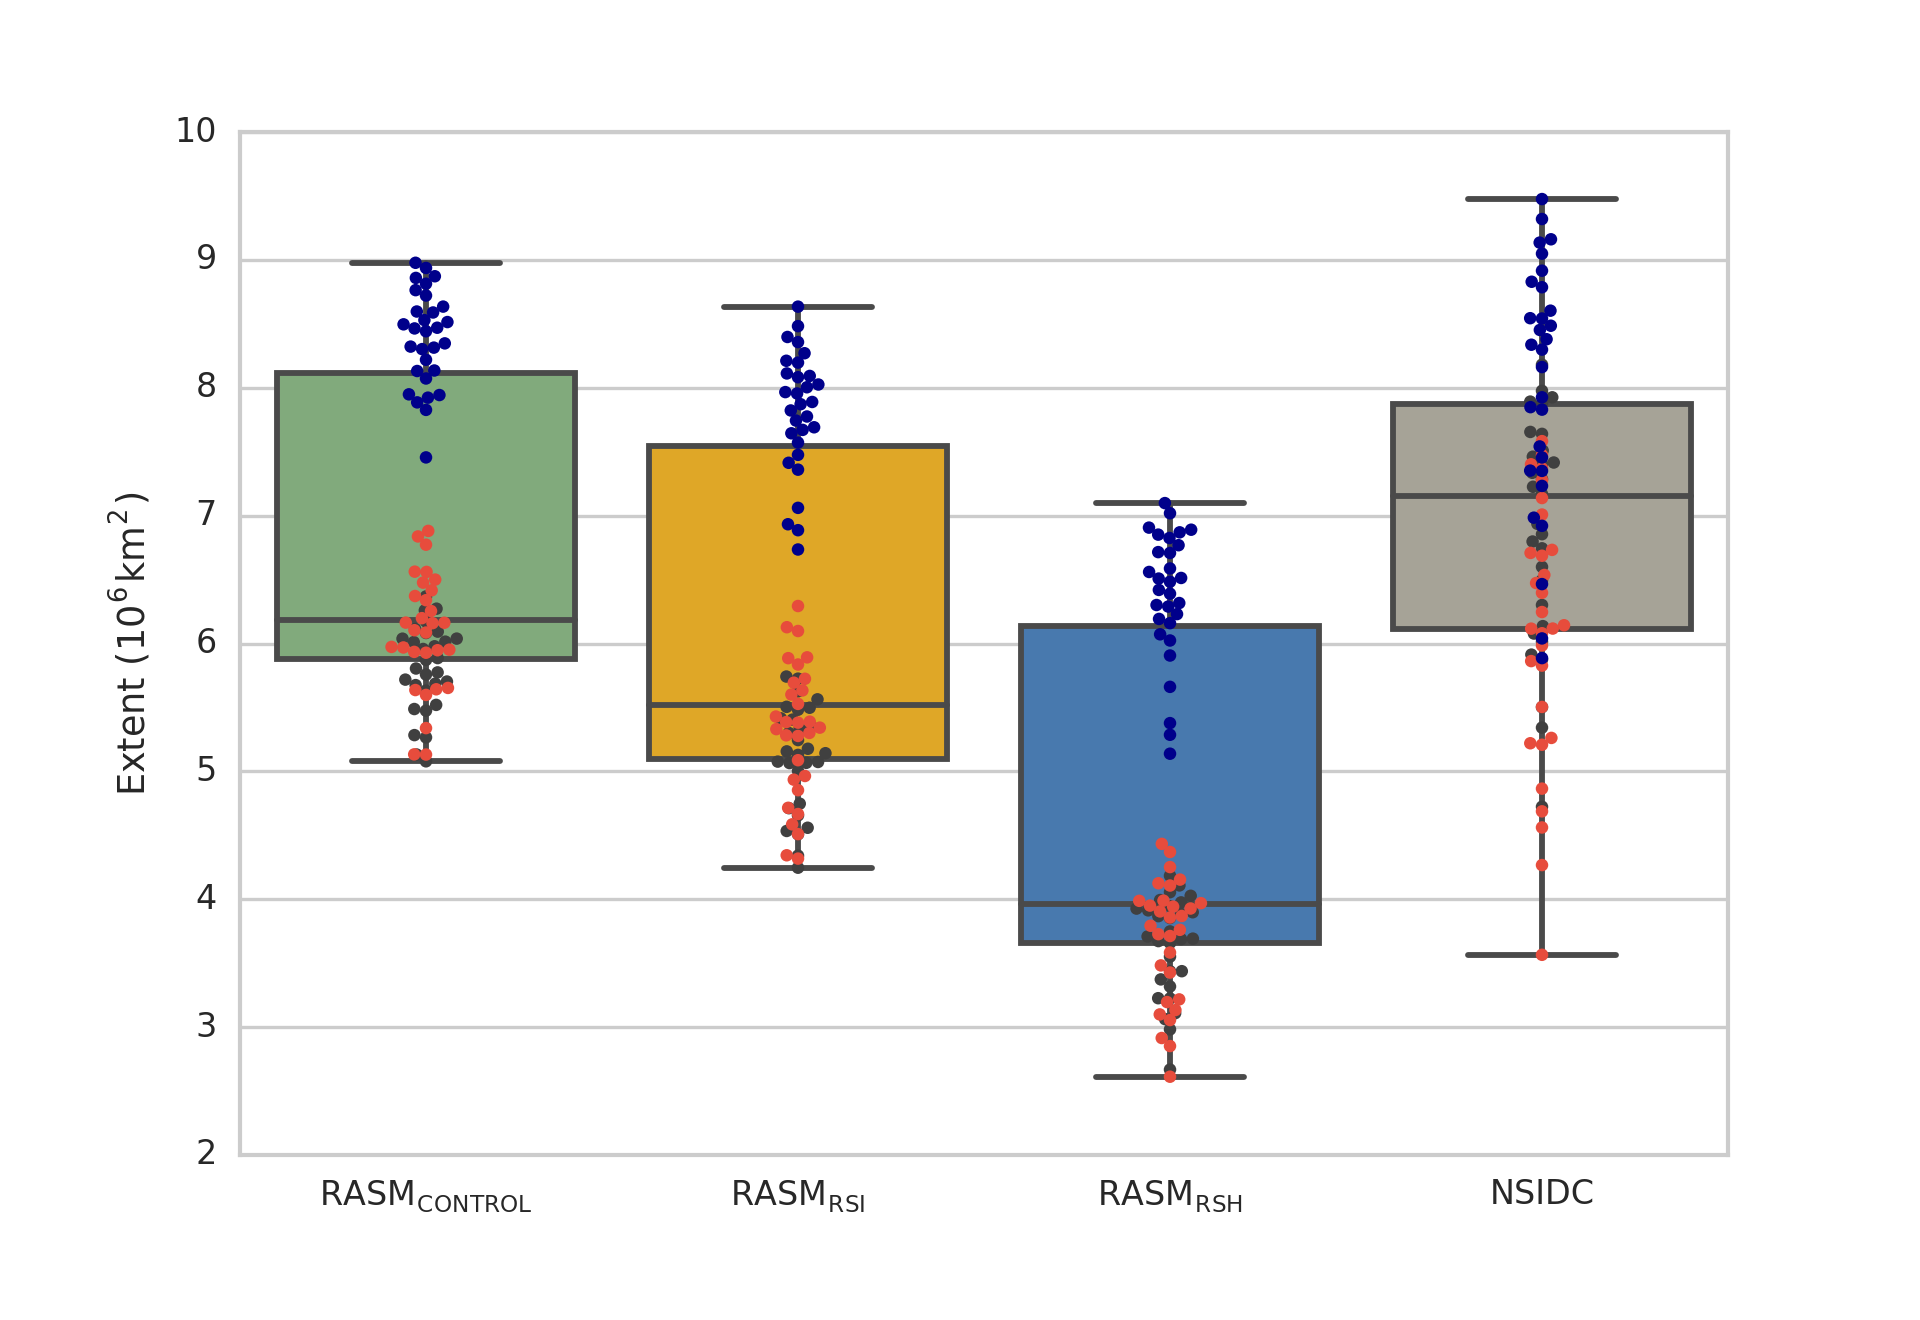
\includegraphics[width=12cm,keepaspectratio]{seaice_boxplots}
  \caption{Distribution of fall (Oct - Dec) sea ice extent in RASM and the NSIDC sea ice index. Time period 1985-2015.}
  \label{fig:sea_ice_box}
\end{figure}

% water budget changes
Figure \ref{fig:fwb} presents the freshwater budget for the three RASM simulations, summarized for the fall months (October-December).
The total moisture convergence for the three simulations are all within 0.05\% of one another, this suggests that changes in .
The reductions in sea ice extent in $RASM_{RSI}$ and $RASM_{RSH}$ are coincident with increases in ocean evaporation of 13\% and 52\%, respectively.
These changes in evaporation from the ocean translate to more modest increases in precipitation over the ocean of 3\% and 11\%.
Associated reductions in convergence over the ocean mask, defined here as P-E between October and December, are found to be 2\% and 10\%. % BN: Is a 2% change meaningful? JH: I'm not sure what you mean.
Finally, while precipitation over land is found to increase relative to the baseline case for both $RASM_{RSI}$ and $RASM_{RSH}$, the increases are relatively small (1\% and 3\% respectively).
These increases in precipitation are sufficient to explain the resulting change in storage (e.g. snow) over land.
Summarizing the water budget, we find that the forced decreases in $RASM_{RSI}$ and $RASM_{RSH}$ lead to significant increases in ocean evaporation but relatively small changes in precipitation over land, despite relatively large changes in ocean evaporation.
Changes in the spatial patterns of precipitation between the three RASM simulations (not shown) lack a regional signal.
While this muted response may be partially explained by the limited interannual variability in the RASM sea ice extent, it also indicates that changes in evaporation from the Arctic Ocean will have to be accompanied with changes in circulation patterns if increases in precipitation are to be attributed to sea ice loss.

\begin{figure}
  \centering
  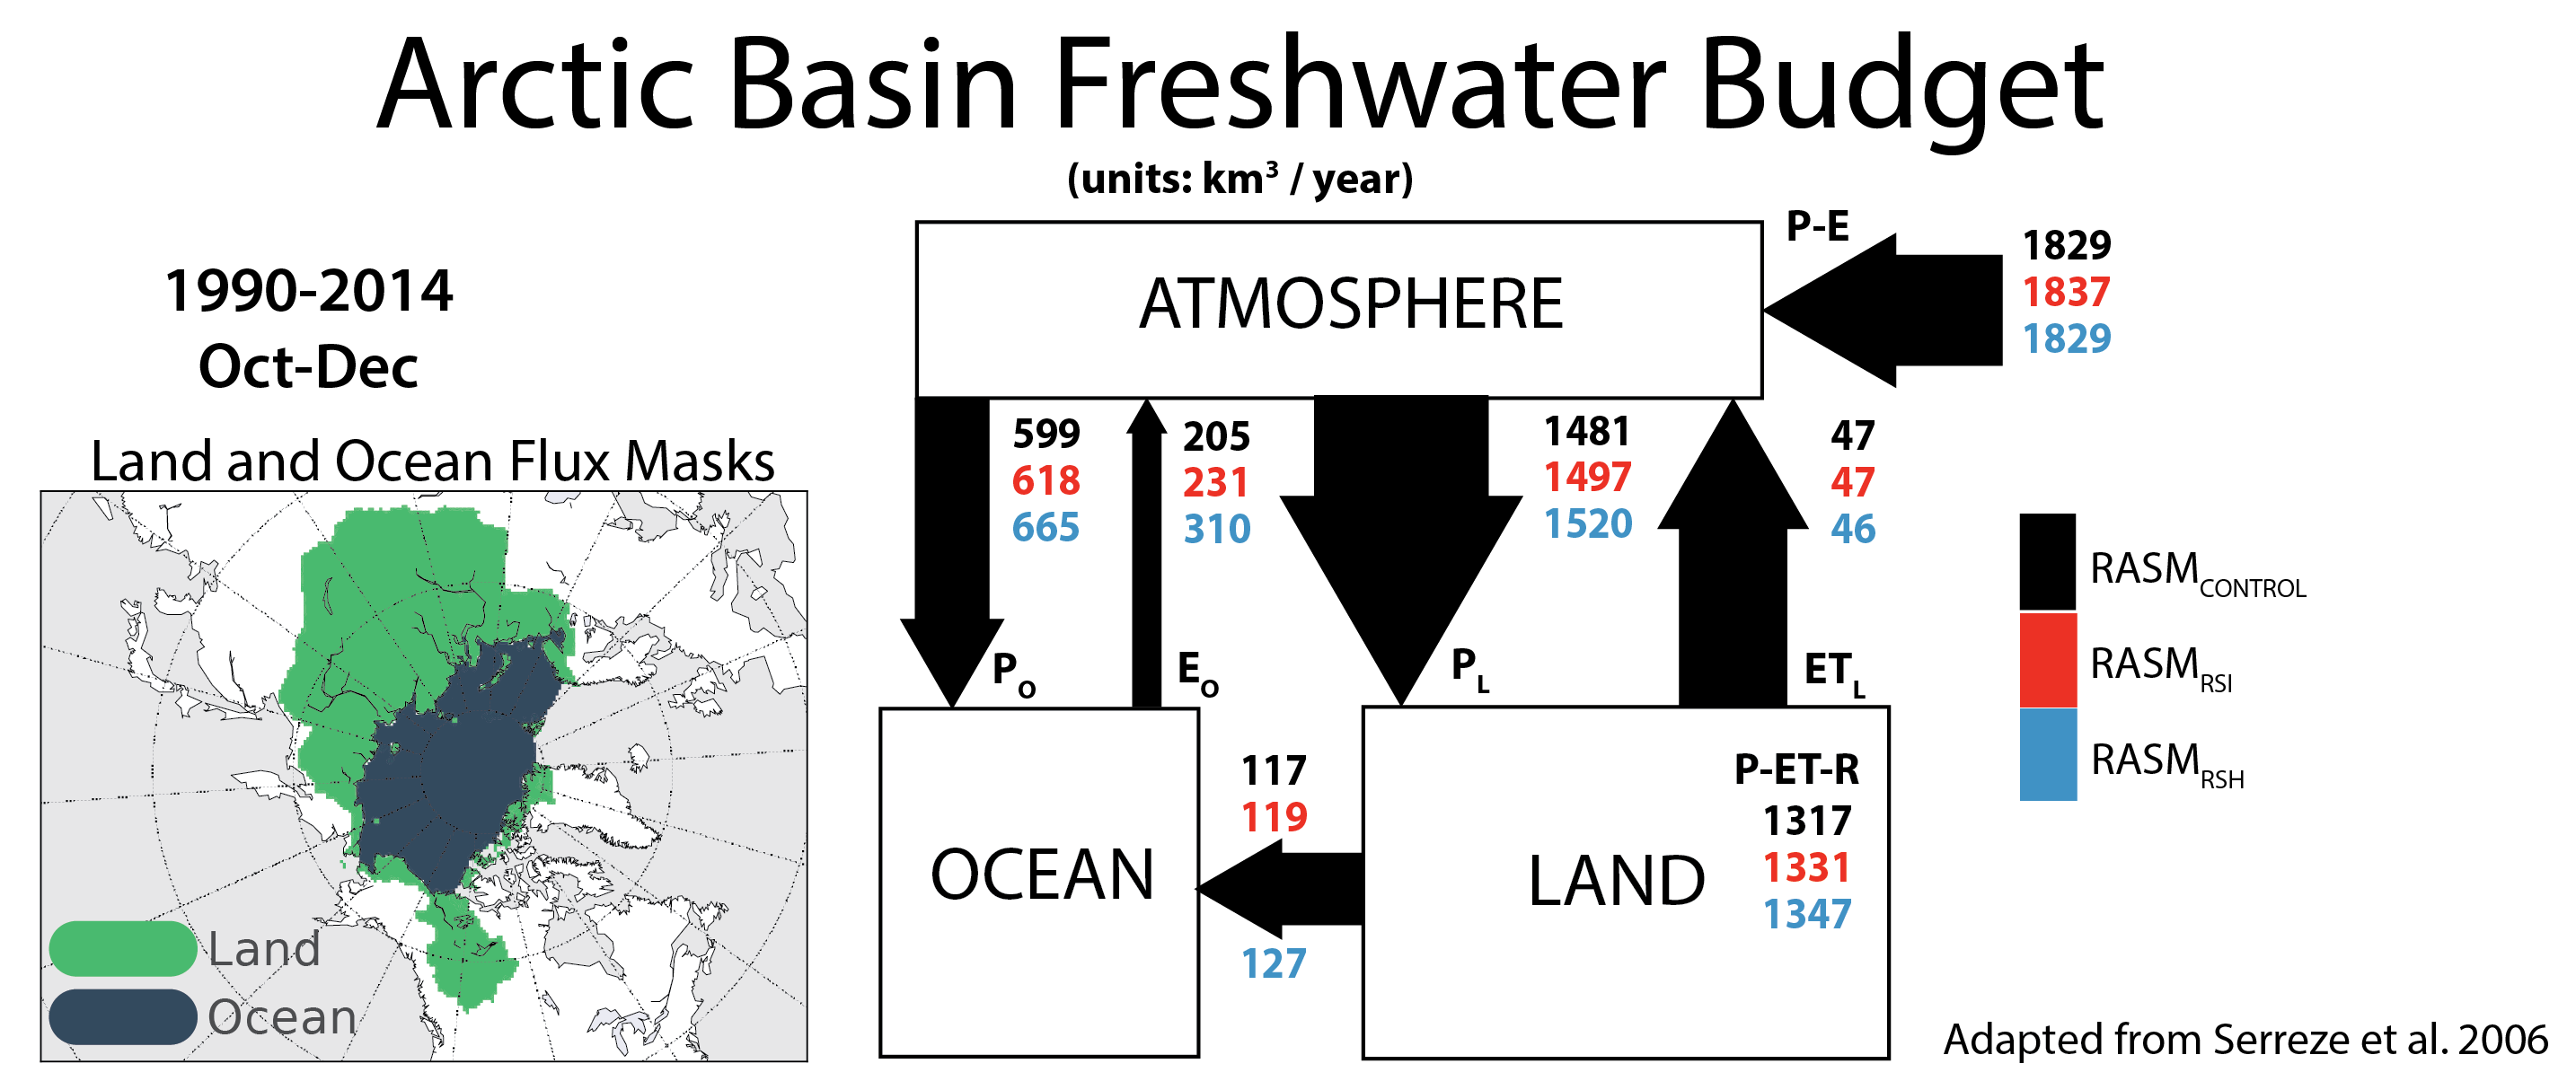
\includegraphics[width=14cm,keepaspectratio]{fresh_water_budget}
  \caption{Arctic freshwater budget, adapted from \citet{Serreze_2006a}.}
  \label{fig:fwb}
\end{figure}

% BN: My main problem with this section is that it reads as if you have found a tool and you are now going to use it just because you have it rather than because you think it may be the best tool for the job. It lacks proper motivation of why you are using SOMs and as a result, the outcomes are rather ambivalent. "I used this technique called SOM and this is what I found". You need to restructure this and provide better motivation for the technique. Rather than being guided by the technique, lead the discussion by what you are interested in (is increased precipitation in the central Arctic a result of a decrease in sea ice extent)? The story is about the latter, not about the technique. Reframing it that way will lead to a better discussion. That starts by removing the "Self-Organizing Maps" as a stand-alone section. It's merely a technique. Focus on the story.
% JH: I've worked to tie the SOM analysis into the story a bit better.

% SOM analysis
We have applied the Self-Organizing Maps technique on standardized evaporation anomalies across the Arctic Ocean to better understand the coupling between ocean sourced evaporation and anomalies in precipitation over land during the fall season.
As we saw in our previous water budget analysis, fairly large relative increases in ocean evaporation led to fairly small changes in precipitation over land.
In applying SOMs, as we do in this section, we will be able to connect regional patterns of ocean evaporation, sea ice, and atmospheric circulation to precipitation patterns over land.

% MASTER SOM
The full, trained Kohonen Layer (or Master SOM) is shown in Figure \ref{fig:master_som}.
The SOM algorithm identified characteristic spatial patterns of evaporation anomalies, with patterns of positive evaporation anomalies toward the top left of Figure \ref{fig:master_som} and patterns of negative evaporation anomalies toward the bottom right.
Here we focus our analysis on four SOM nodes that exhibit the largest hit rate (number of months in a particular pattern) and evaporation patterns of interest: (0,1), (0,3), (1,0), and (1,2).
We will show that the first two SOMs represent generally wet patterns (high precipitation) while the second two represent generally dry patterns (low precipitation) by mapping these patterns to their coincident patterns of precipitation.
In each of these patterns, the combined position, sign, and magnitude of evaporation anomalies in the central Arctic, Kara/Barents sea, and North Atlantic Ocean are characteristically different.

\begin{figure}
  \centering
  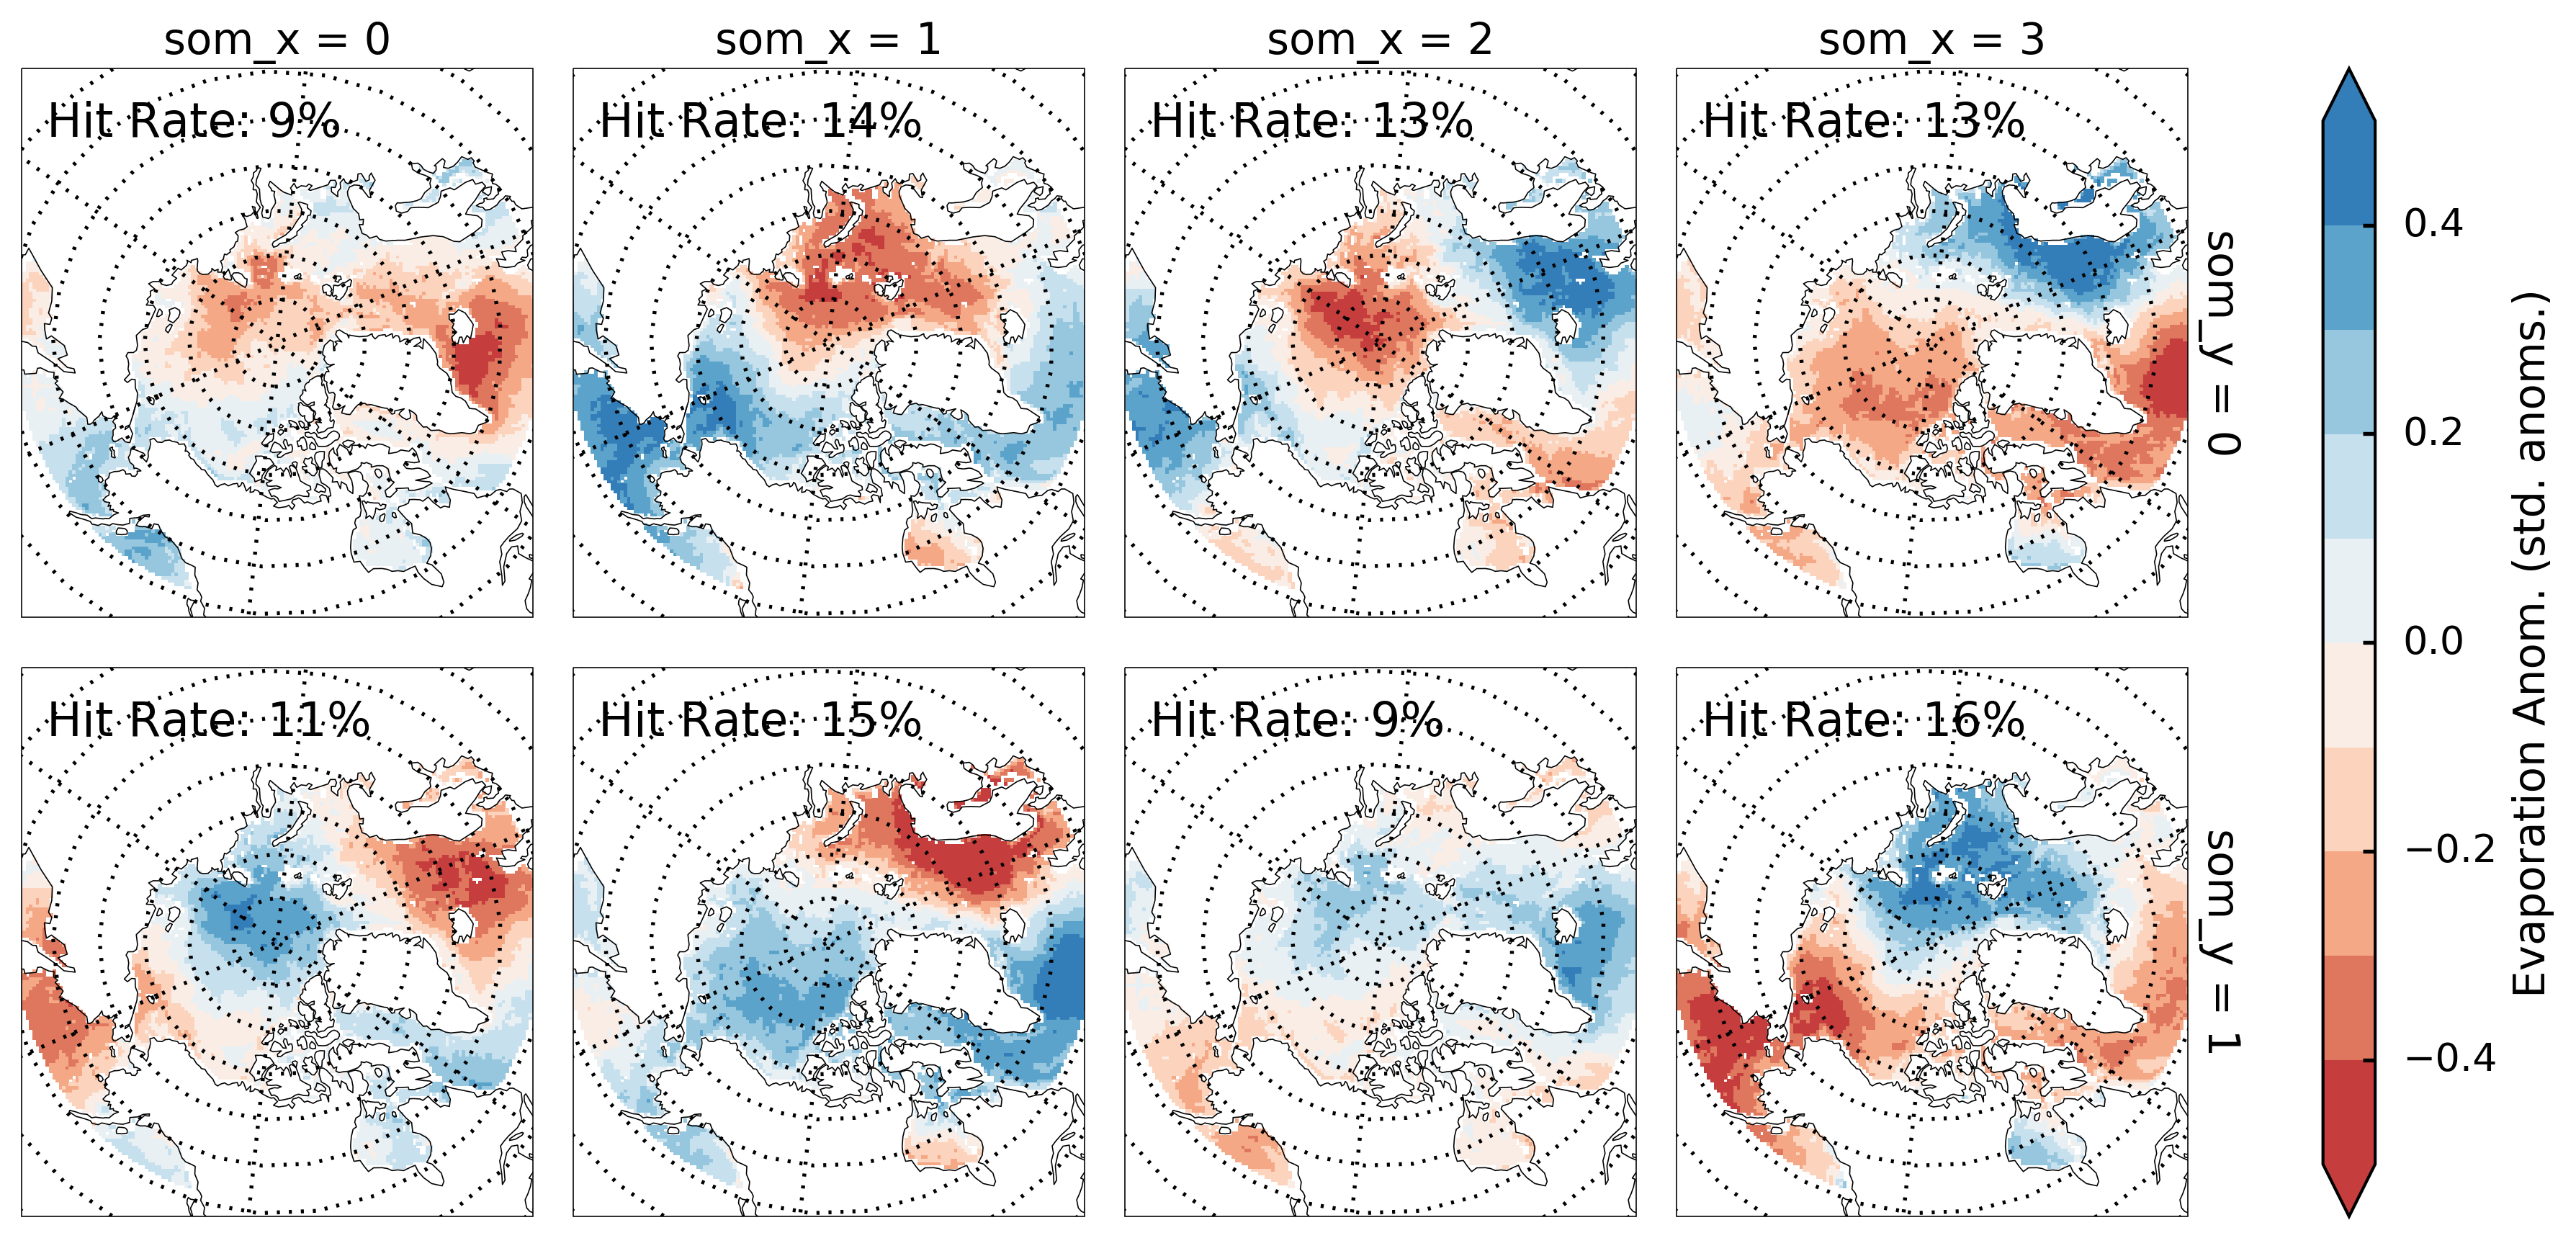
\includegraphics[width=14cm,keepaspectratio]{master_som}
  \caption{Master SOM. The hit rate, shown as the percentage of all the months (270) in the training dataset in each pattern, is shown in the top left corner.}
  \label{fig:master_som}
\end{figure}

% Composite SOM
Figure \ref{fig:composite_som} presents the mapped fields for the four SOM nodes discussed above.
Each of the mapped fields represent the composite mean of all months assigned to SOM node.
Here we focus on ocean evaporation, sea level pressure (SLP), sea ice concentration, precipitation over land, and snow water equivalent.
For node (0,1), anomalously high evaporation rates from the North Atlantic are accompanied by anomalously low pressure in the region.
This combination is found to lead to positive precipitation anomalies over Northern Europe.
Node (0,3) exhibits positive evaporation anomalies in the Kara and Barents Seas and negative evaporation anomalies in the North Atlantic.
SLPs for this node are anomalously high across North America from Alaska to Greenland, indicating a southward shift of the storm track.
Corresponding precipitation anomalies for node (0,3) are positive over eastern Europe and central Siberia.
Neither of the wet nodes have sea ice concentration anomalies that can be clearly tied to evaporation or precipitation anomalies.
The lack of correspondence between sea ice and evaporation anomalies indicates that variability in the fall evaporation flux in RASM is largely being driven by patterns in the ocean and atmosphere.

\begin{figure}
  \centering
  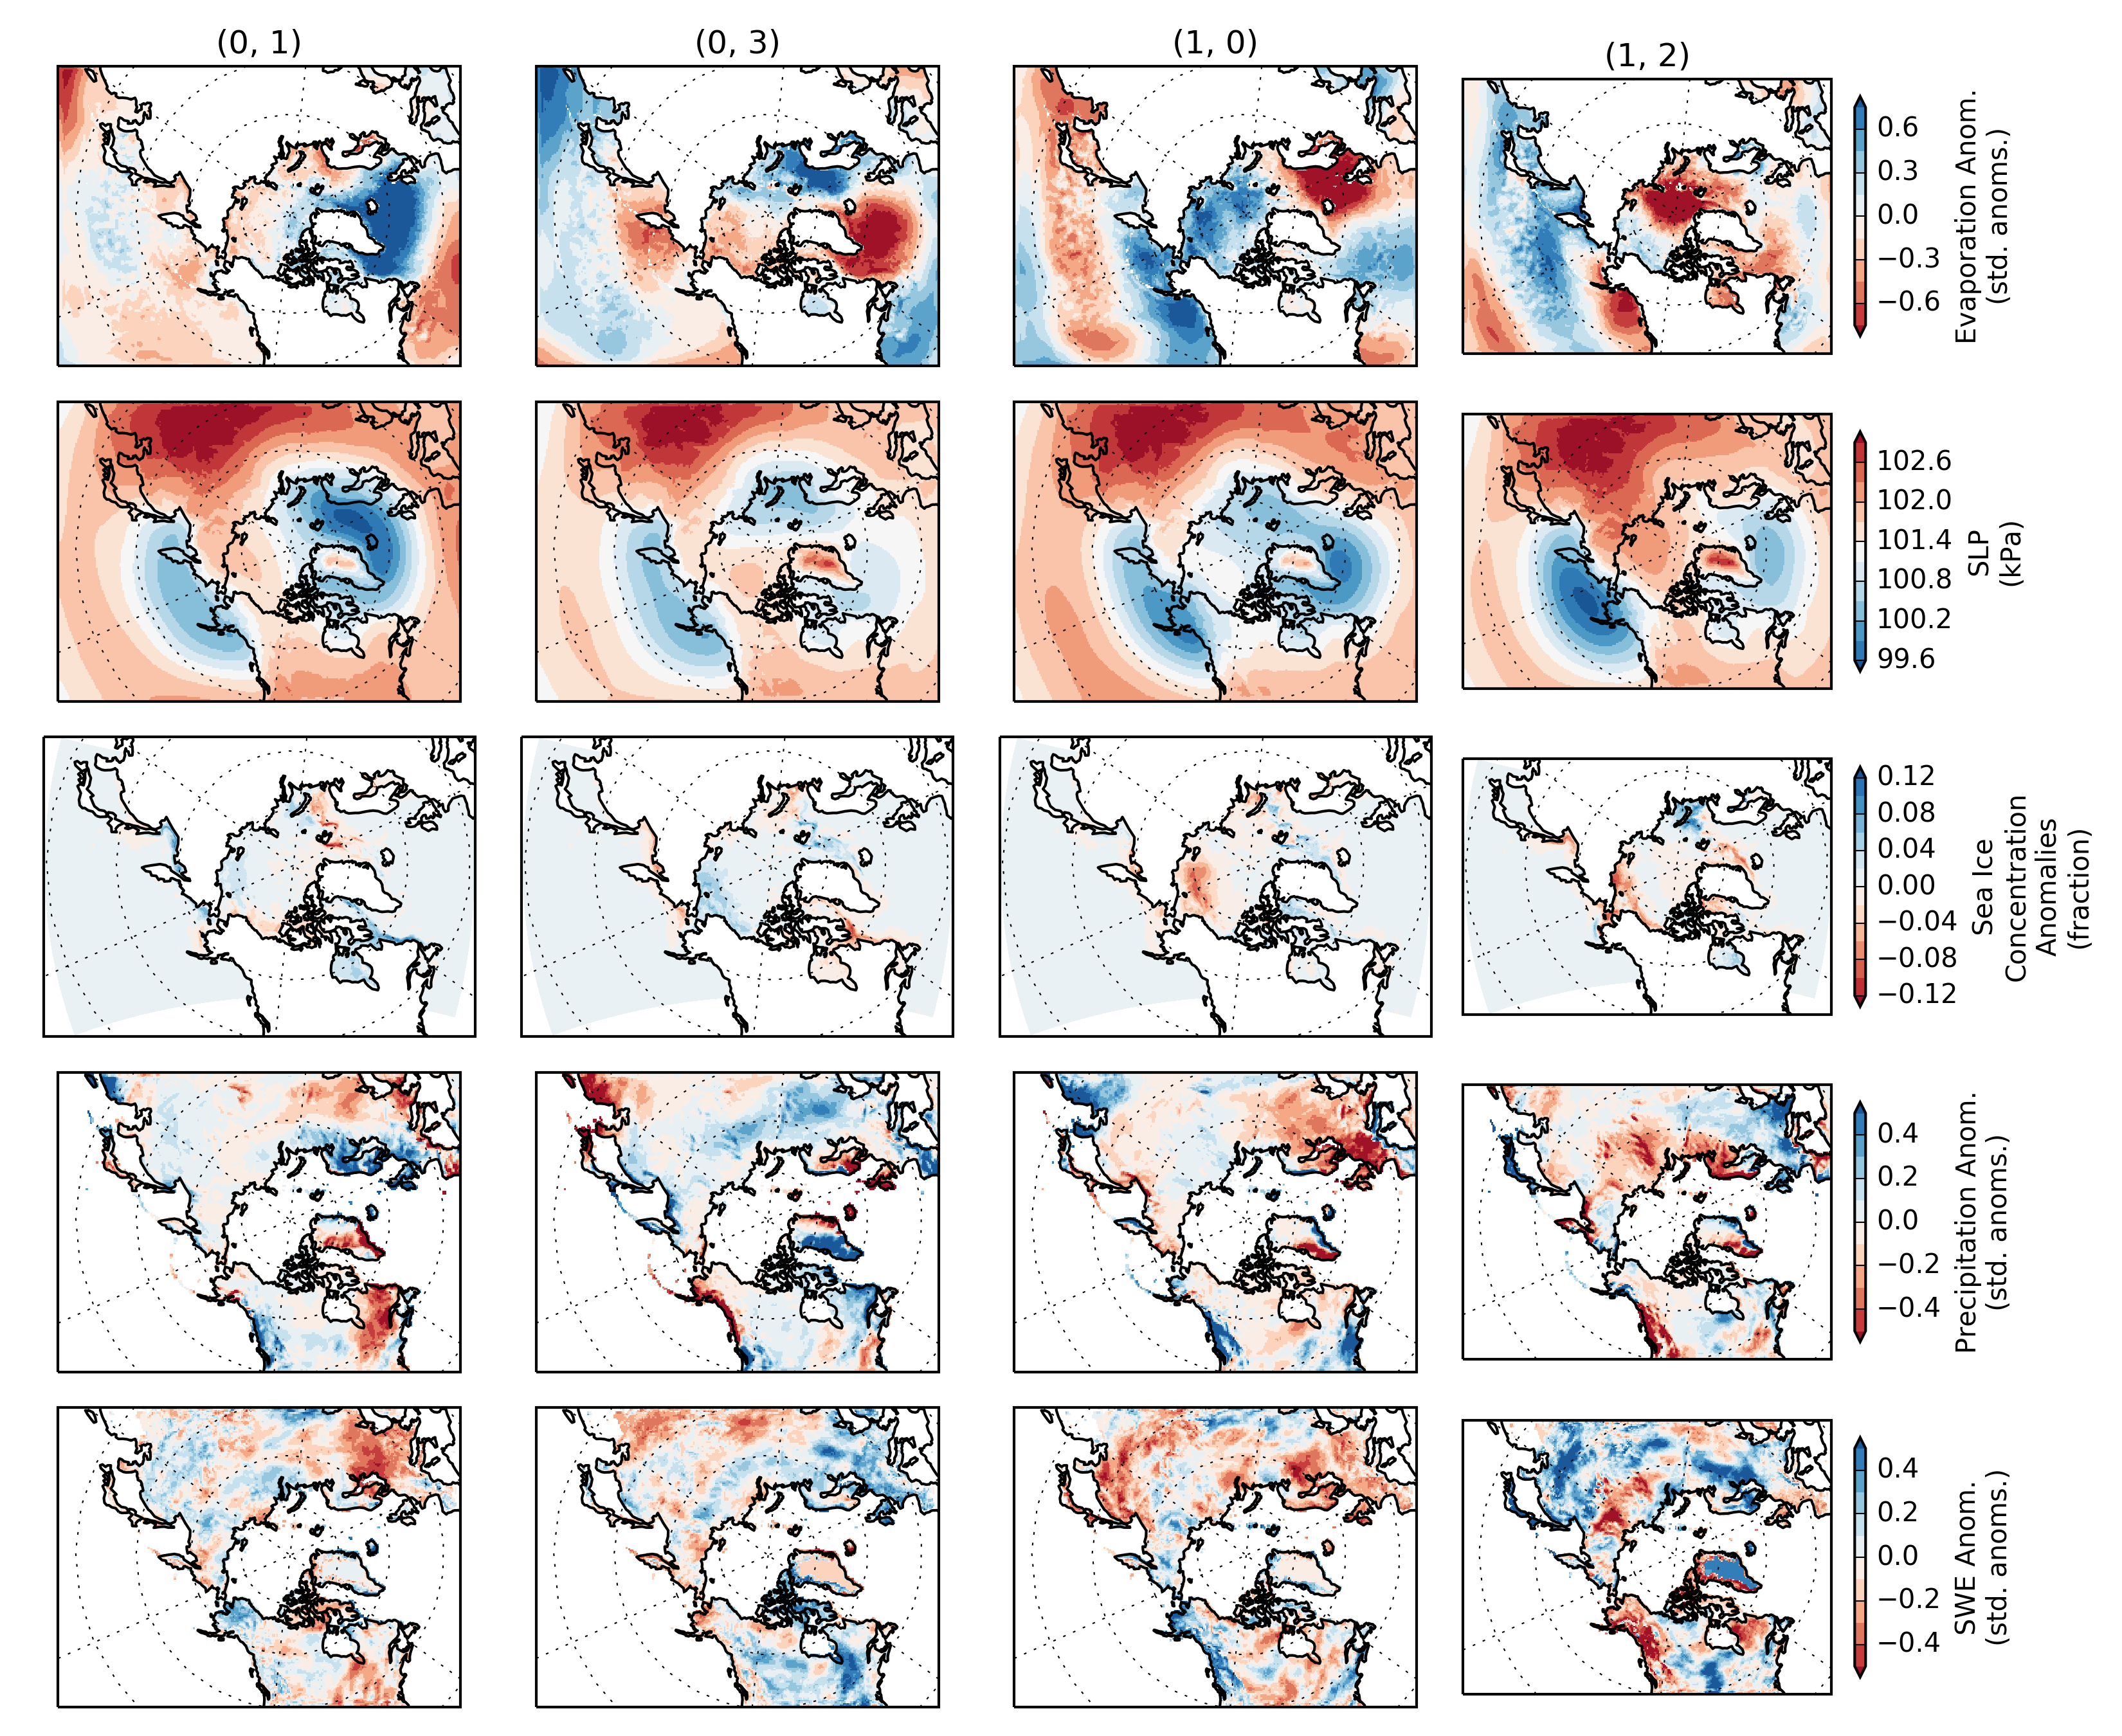
\includegraphics[width=15cm,keepaspectratio]{composite_som}
  \caption{SOM nodes (0,1), (0,3), (1,0), and (1,2) mapped to ocean evaporation, sea level pressure (SLP), sea ice concentration, precipitation over land, and snow water equivalent. Except for sea level pressure, values plotted are the average anomalies across all the members of each node.}
  \label{fig:composite_som}
  % BN: I don't know how to interpret the ET units
  % BN: Should this analysis be limited to the Central Arctic?
\end{figure}
% TODO: get the subplots to align better

The selected dry nodes, (1,0) and (1,2), are characterized by negative evaporation anomalies east and north of Greenland, respectively, and positive anomalies in the central Arctic and Siberian Shelf.
Both nodes are mapped to negative sea ice concentration anomalies along the Siberian Shelf.
In node (1,2), positive sea ice concentration anomalies in the Kara Sea correspond to the negative anomalies ocean evaporation, although the spatial extent is considerable larger in the evaporation anomalies.
Node (1,2) also includes positive SLP anomalies across the central Arctic.

% Hit Map
The trained SOM can be used to identify the frequency of occurrence of each pattern as a function of month (October, November, or December) and RASM simulation ($RASM_{CONTROL}$, $RASM_{RSI}$, or $RASM_{RSH}$).
Figure \ref{fig:som_hit_freq} plots the mapping frequency, by month and simulation, for each node in the 2x4 SOM.
Node (0,1), which has a large region of positive evaporation anomalies across the North Atlantic, occurs nearly twice as frequently in $RASM_{RSH}$ as in $RASM_{CONTROL}$.
The opposite is found in node (0,3), where the hit frequency is found to decrease under reduced sea ice conditions.
Interestingly, the hit frequency for dry nodes [e.g. (1,0) and (1,2)] is mostly stable between the simulations.
On the whole, the SOM analysis indicates that decreasing sea ice extent and the associated evaporation changes are most likely to contribute to wetting trends over land when these changes are accompanied by a shift in atmospheric circulation [e.g. node (0,3)].
Global climate models tend to suggest that future Arctic climate will be stormier \citep{Vavrus_2012} and that winter circulation patters may trend toward a more variable pattern.
However, the fact that the patterns with large shifts in frequency [(0,1) and (1,2)] shift in directions that limit the impact of sea ice loss, indicates that the precipitation response may be dampened.

\begin{figure}
  \centering
  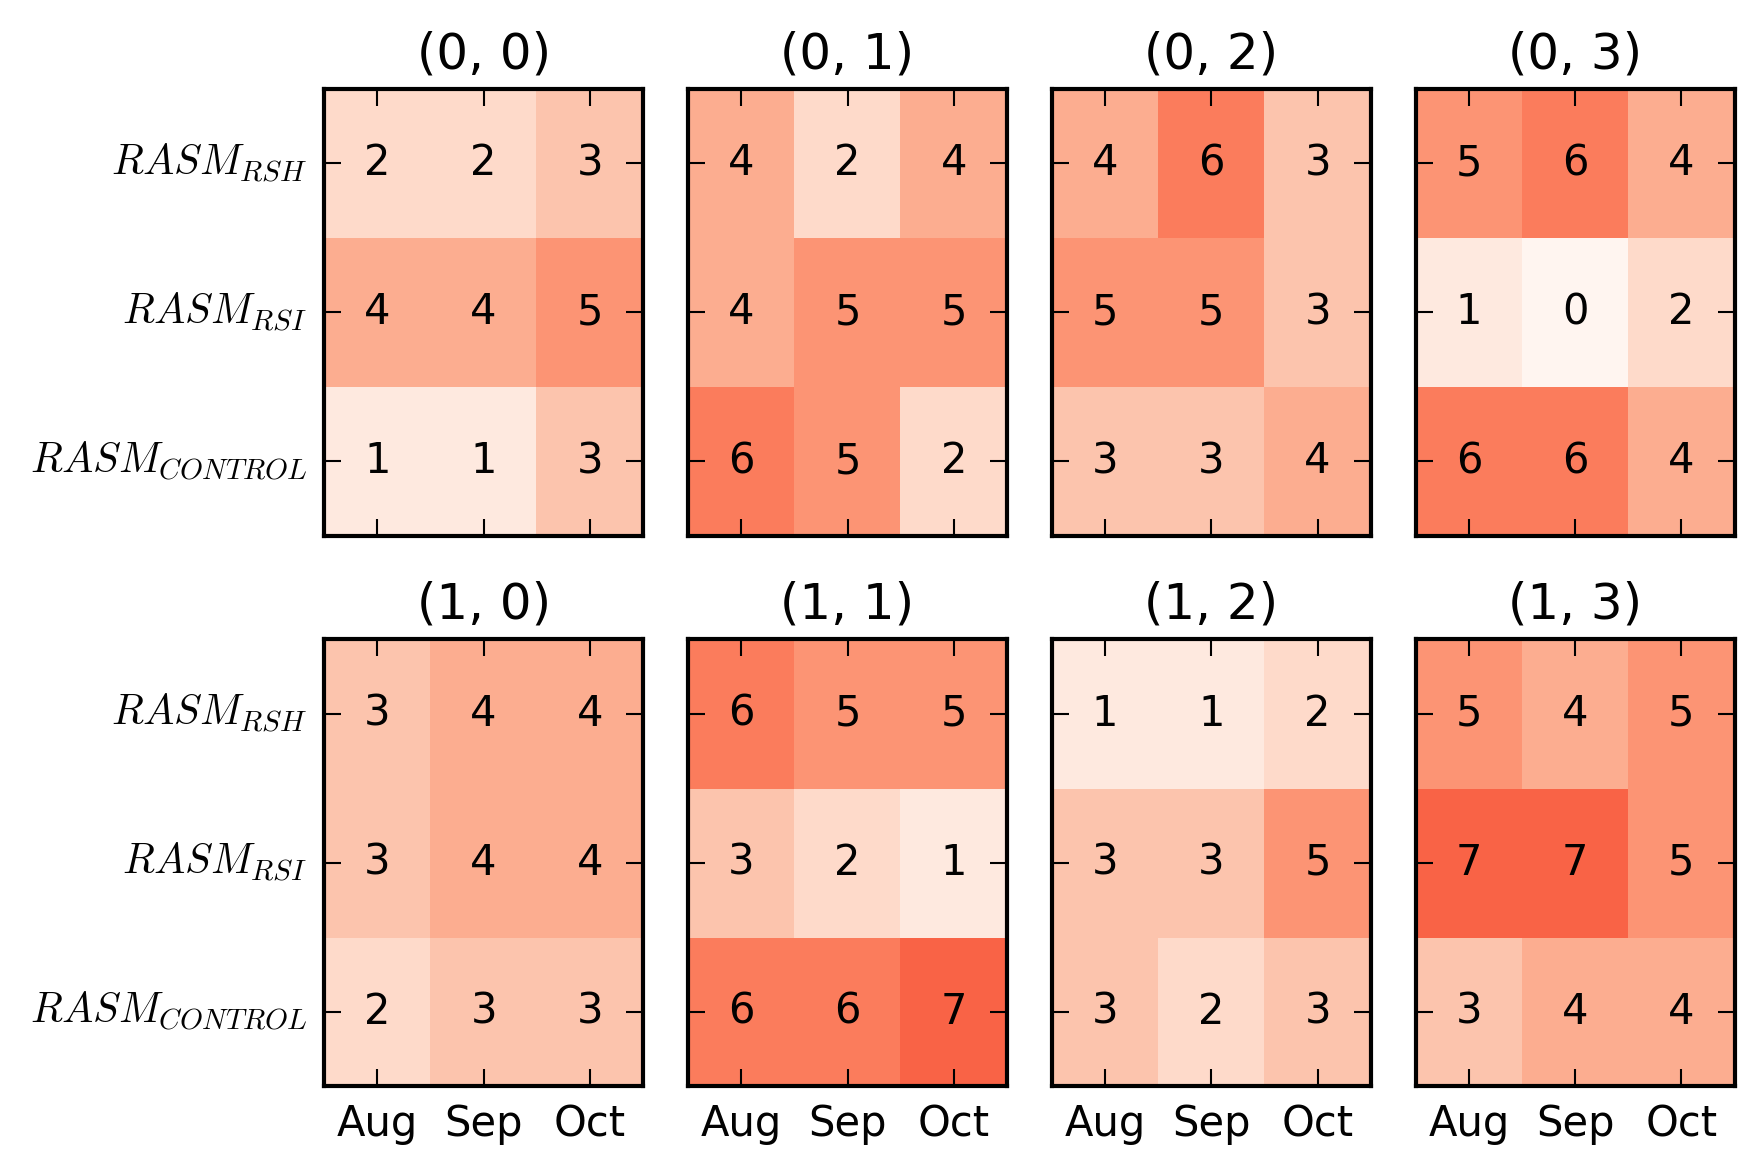
\includegraphics[width=10cm,keepaspectratio]{som_hit_freq}
  \caption{SOM hit frequency by month and RASM simulation.}
  \label{fig:som_hit_freq}
\end{figure}

\section{Conclusions}
\label{sec:conclusions_ch5}

We have investigated the relationship between sea ice extent and early winter precipitation over the Pan Arctic land masses.
We have demonstrated observed interannual covariation between sea ice extent and precipitation over land.
Our initial hypothesis was that variations in sea ice extent were a driving factor in precipitation over land in the fall.
A water budget analysis highlighted that although relatively large changes in winter evaporation from the Arctic Ocean are expected (50\% in our simulation with the lowest sea ice concentration), these changes are proportionally small when compared to the precipitation flux over land.
Furthermore, the modest increases in terrestrial fall season precipitation simulated by RASM under reduced sea ice conditions indicate that there will have to be significant circulation changes in the future if ocean sourced evaporation is likely to significantly impact precipitation over land.
Our SOM analysis has also pointed us in this direction, which is that the ties between evaporation and precipitation are only robust under certain atmospheric circulations.
Across Eurasia, the dominant coupling between precipitation and Arctic Ocean evaporation requires low pressure anomalies over the central Arctic, similar to the negative phase of the Arctic Oscillation \citep{Thompson_1998}.
Previous work by \citet{Cassano_2014}, using partially coupled global simulations with prescribed sea ice, has also indicated that reductions in sea ice extent in the fall may contribute negative sea level pressure anomalies over the Arctic Ocean.


Of particular interest is the sea ice state in the Kara and Barents Seas.
As sea ice declines, we expect that this coupling will become stronger, especially if the Arctic is to become stormier.
We have found that sea ice retreat along the Siberian shelf and north Alaskan coast is holds less influence on precipitation regional patterns.
In these areas, the circulation patterns (low pressure in North Pacific) tend to limit the influence of enhanced evaporation along the retreating ice edge.
